%
% disk.tex -- normal derivative on disk boundary
%
% (c) 2019 Prof Dr Andreas Müller, Hochschule Rapperswil
%
\documentclass[tikz,12pt]{standalone}
\usepackage{amsmath}
\usepackage{times}
\usepackage{txfonts}
\usepackage{pgfplots}
\usepackage{csvsimple}
\usetikzlibrary{arrows,intersections,math}
\begin{document}
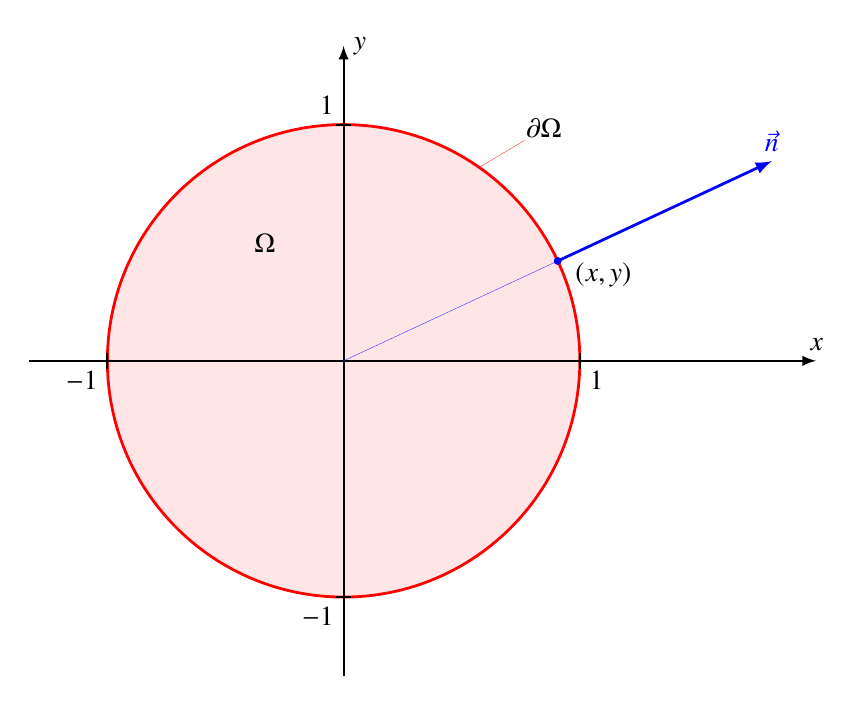
\begin{tikzpicture}[>=latex]

\fill[color=red!10] (0,0) circle[radius=3];
\draw[color=red,line width=1pt] circle[radius=3];

\draw[->,line width=0.7pt] (-4,0)--(6,0) coordinate[label={$x$}];
\draw[->,line width=0.7pt] (0,-4)--(0,4) coordinate[label={right:$y$}];

\def\a{25}
\def\b{55}

\draw[->,line width=1pt,color=blue] ({3*cos(\a)},{3*sin(\a)})--
	({6*cos(\a)},{6*sin(\a)});
\fill[color=blue] ({3*cos(\a)},{3*sin(\a)}) circle[radius=0.05];
\node[color=blue] at ({6*cos(\a)},{6*sin(\a)}) [above] {$\vec{n}$};

\draw[line width=0.1pt,color=blue] (0,0)--({3*cos(\a)},{3*sin(\a)});

\draw[line width=0.7pt] (3,-0.1)--(3,0.1);
\node at (3,0) [below right] {$1$};
\draw[line width=0.7pt] (-3,-0.1)--(-3,0.1);
\node at (-3,0) [below left] {$-1$};
\draw[line width=0.7pt] (-0.1,3)--(0.1,3);
\node at (0,3) [above left] {$1$};
\draw[line width=0.7pt] (-0.1,-3)--(0.1,-3);
\node at (0,-3) [below left] {$-1$};

\node at (-1,1.5) {$\Omega$};
\draw[line width=0.1pt,color=red] ({3*cos(\b)},{3*sin(\b)})--(2.3,2.8);
\node at (2.2,2.7) [above right] {$\partial\Omega$};

\node at ({3*cos(\a)+0.1},{3*sin(\a)+0.1}) [below right] {$(x,y)$};

\end{tikzpicture}
\end{document}

